\documentclass[a4paper]{article}

%%%%%%%%%%%%%%%%%%%%%%%%%%%%%%%%%% 
% Package for making LaTeX properly handle utf8 characters set and danish language rules
\usepackage[utf8]{inputenc}
\usepackage[danish]{babel}

%%%%%%%%%%%%%%%%%%%%%%%%%%%%%%%%%% 
% Package for changing to a nicer font 
\usepackage[T1]{fontenc}

%%%%%%%%%%%%%%%%%%%%%%%%%%%%%%%%%% 
% Package for conctroling the text area
\usepackage[margin=2.5cm]{geometry}

%%%%%%%%%%%%%%%%%%%%%%%%%%%%%%%%%% 
% Package for inserting clickable hyperlinks in pdf versions as produced by pdflatex
\usepackage{enumitem, hyperref}

%%%%%%%%%%%%%%%%%%%%%%%%%%%%%%%%%% 
% Package for including figures. TeX and thus LaTeX was developped before the existence of directory file-structures, but the graphicspath let's you add directories, that the \includegraphics will search.
\usepackage{graphicx}
\graphicspath{{figures/}}

%%%%%%%%%%%%%%%%%%%%%%%%%%%%%%%%%% 
% Package for typesetting programs. Listings does not support fsharp, but a little modification goes a long way
\usepackage{listings}
\usepackage{xcolor}
\usepackage{verbatim}
\usepackage{color}
\usepackage{textcomp}

\renewcommand{\figurename}{Figur}
\renewcommand{\contentsname}{Indholdsfortegnelse}
\renewcommand{\contentsname}{Table of Contents}
\renewcommand{\lstlistingname}{Kodestykke}
\renewcommand{\partname}{Afsnit}

\def\sectionautorefname~#1\null{%
  Afsnit #1\null
}

\def\subsectionautorefname~#1\null{%
  Afsnit #1\null
}

\def\figureautorefname~#1\null{%
  Figur #1\null
}

\def\equationautorefname~#1\null{%
  Ligning #1\null
}

\def\namedlabel#1#2{\begingroup
    #2%
    \def\@currentlabel{#2}%
    \phantomsection\label{#1}\endgroup
}

\definecolor{bluekeywords}{rgb}{0.13,0.13,1}
\definecolor{greencomments}{rgb}{0,0.5,0}
\definecolor{turqusnumbers}{rgb}{0.17,0.57,0.69}
\definecolor{redstrings}{rgb}{0.5,0,0}
\definecolor{lightgray}{RGB}{240, 240, 240}

\newcommand{\namedref}[1]{\autoref{#1} - \nameref{#1}}

\lstdefinelanguage{FSharp}
				{morekeywords={\#load, \#r, let, new, match, with, rec, open, module, namespace, type, of, member, and, for, in, do, begin, end, fun, function, try, mutable, if, then, else, List, Set, Sudoku, Seq, false, true, Assert, printfn, print, sprintf, when, ->, >, ::, printf, yield},
	keywordstyle=\color{bluekeywords},
	sensitive=false,
	morecomment=[l][\color{greencomments}]{///},
	morecomment=[l][\color{greencomments}]{//},
	morecomment=[s][\color{greencomments}]{{(*}{*)}},
	morestring=[b]",
	stringstyle=\color{redstrings},
	tabsize=2, % sets default tabsize to 2 spaces
	backgroundcolor=\color{lightgray}
}

\usepackage[table]{}
\usepackage{array}
\usepackage{algorithm}
\usepackage{caption}
\usepackage{float}
\usepackage{amsmath}
\usepackage{algorithm}
\usepackage[noend]{algpseudocode}
\usepackage{mathtools}
\usepackage{ragged2e}
\usepackage{caption}
\usepackage{amssymb}
\usepackage{listingsutf8}
\usepackage{newunicodechar}
\usepackage{nameref}
%\newunicodechar{┌}{?}

% Site med mange eksempler - både kode og billeder
% http://www.texample.net/tikz/

%%% Tikz: pakke til at lave grafik
\usepackage{tikz}

\usepackage{url}

%%% Tilføjer makroer der gør livet lettere for os
\usetikzlibrary{arrows, shapes, positioning}

%%% Pile
%%% http://www.texample.net/media/pgf/builds/pgfmanualCVS2012-11-04.pdf (afsnit 24)
\tikzset{
  aggr/.style={->, >=open diamond},
  inh/.style={->, >=open triangle 45}
} 

%%% Bokse
%%% http://www.texample.net/media/pgf/builds/pgfmanualCVS2012-11-04.pdf (afsnit 49)
\tikzset{
  class/.style={draw, rectangle}
}

\lstset{ %
  numbers=right,                    % where to put the line-numbers; possible values are (none, left, right)
  numbersep=5pt,                   % how far the line-numbers are from the code
  numberstyle=\small\color{bluekeywords}, % the style that is used for the line-numbers
  stepnumber=1,                    % the step between two line-numbers. If it's 1, each line will be numbered
  title=\lstname,                   % show the filename of files included with \lstinputlisting; also try caption instead of title
  showstringspaces=false,
  breaklines=true,
  captionpos=b,
  language=FSharp,
  texcl=true,
  inputencoding=utf8,
  extendedchars=true,
  mathescape=true,
  %escapeinside={(*}{*)},
  literate=
	{æ}{{\ae}}1
	{å}{{\aa}}1
	{ø}{{\o}}1
	{Æ}{{\AE}}1
	{Å}{{\AA}}1
	{Ø}{{\O}}1
	{ü}{{\"u}}1
	{├}{{?}}1
	{┐}{{?}}1
	{┌}{{?}}1
	{┘}{{?}}1
	{└}{{?}}1
	{╞}{{?}}1
	{╪}{{?}}1
	{╬}{{?}}1
	{┌}{{?}}1
	{┼}{{?}}1
}

\setlength\parindent{0pt}

\title{Simple Jack - Programmering og Problemløsning}
\author{Mads U. Svendsen, Anders F. Jørgensen, Nicolai L. Hargreave, Bo H. Thomsen}

\begin{document}
	\maketitle % Insert title etc.
        
  \tableofcontents

  \newpage

\section{Forord}
    
\section{Introduktion} \label{sec:introduction}
    Denne opgave er lavet i Programmering og Problemløsning(PoP),
    på Datalogisk Institut - Københavns Universitet(DIKU).
    Opgaven har opgavenummeret 10g, målet for opgaven er at
    udvikle en spilbar version af spillet SimpleJack.

    \paragraph*{Sådan kompilerer du projektet\\}
    I \path{/src} mappen ligger der en Makefile og hvis man kører den, 
    kompileres \lstinline$game.exe$,
    begge filer kan findes i mappen \path{/src}.
    Kommandoen til at kompilerer er  \lstinline$make$ og kan den kan skrives i terminalen.

    Derudover kan man kompilerer projektet med dokumentation, ved at bruge kommandoen \lstinline$make withdocs$

    Tests findes i  mappen \path{/src}, i filen \lstinline$tests.fsx$,
    og kan kompileres med \lstinline$fsharpc$ og køres med \lstinline$mono$.

\newpage

\section{Problemformulering} \label{sec:problem}
  I dette afsnit vil vi introducere det problem vi ønsker at løse med programmet,
  og beskrive hvordan vi har forstået den udleverede kravspecifikation.

  I dette projekt vil vi gerne udvikle et program der kan spilles af 1-5 spillere i kommandoprompten,
  med mulighed for AI. Programmet er implementeret i F\# og følger reglerne for SimpleJack der er beskrevet i afsnit \ref{ssec:demands} - \nameref{ssec:demands}.

  \subsection{Kravspecifikation} \label{ssec:demands}
    Undervisningforløbet hvorigennem dette projekt udfodler sig, er der fokus på klasser og objekter,
    via ement ”\textit{Object Orienteret Programmering}” (OOP).
    Et af kravene, er defor at progammet skal være designet efter det objekt-orienteret paradigme.
    Hertil kommer, at projektet skal planlægges gennem bl.a. et UML diagram.

    Herunder er kravene til det færdige produkt opstillet, hvorved det er beskrevet hvordan kravene fra projektoplægget er blevet fortolket.

    \begin{enumerate}
      \item I SimpleJack spilles ikke om penge/jetoner men om sejr/tab, mellem spiller(e) og dealer.\\
            Hvilket i opgaven er opfattet som en/et enkelt sejr/nederlag; hvorefter spillet kan 
            starte fra ny.
      \item SimpleJack består af en dealer og 1-5 spillere
      \item Der bruges et normalt kortspil (uden jokere), altså 13x4 = 52 kort
      \item Ved spilstart får dealer og hver spiller 2 tilfælde kort fra bunken,
      med billedsiden opad - så værdien er synlig for alle
      \item Hver spiller har en tur, og dealeren har altid tur til sidst
    \end{enumerate}

    Kortværdierne i spillet er fordel efter følgende princip:
    \begin{enumerate}
      \item Billedkort (knægt, dame og konge) har alle værdien 10
      \item Et es kan enten have værdien 1 eller 11
      \item Kort mellem 2 og 10 har den påtrygte værdi
    \end{enumerate}

    Hver spiller, spiller et individuelt spil med dealeren,
    hvor det gælder om at ende med en sum af kortenes værdier er højere end dealerens sum. Hvis summen overstiger 21 er deltageren "bust" og har tabt.
    Fordi hver spiller, spiller et individuelt spil kan alle sagtens vinde.

    Når en spiller har tur, skal en af de følgende handlinger udføres:
    \begin{enumerate}
      \item "Stand": Spilleren/dealeren vælger at give sin tur videre
      \item "Hit": Spilleren/dealeren modtager et kort ad gangen fra bunken,
      indtil han/hun stopper sin tur
    \end{enumerate}

    En spiller har vundet hvis ingen af følgende er gældende:
    \begin{enumerate}
      \item Spilleren er "bust"
      \item Spillerens hånd har en sum der er lavere eller lig med,
      summen af dealerens hånd
      \item Både spilleren og dealeren har SimpleJack(Es og et billedkort)
    \end{enumerate}

    En spiller kan enten deltage i spillet via terminalen,
    eller en spiller kan være en AI som følger følgende regler(Opgavebeskrivelsen):
    \begin{enumerate}
      \item Vælg altid "Hit", medmindre summen af egne kort kan være 17 eller over, ellers vælg "Stand"
      \item Vælg tilfældigt mellem "Hit"og "Stand". Hvis "Hit"vælges trækkes et kort og der vælges igen tilfældigt mellem "Hit"og "Stand"osv.
    \end{enumerate}
  \newpage

  \section{Problemanalyse og design} \label{sec:design}
    I dette afsnit vil vi beskrive hvilken struktur vi har tænkt os at opbygge vores programefter.
    Vi vil introducere et UML diagram og beskrive de tanker der ligger bag vores designvalg.

    \subsection*{Struktur}
      Vores design bygger op omkring fire kerne klasser,
      \texttt{Game}, \texttt{\texttt{Player}}, \texttt{\texttt{Hand}} og \texttt{\texttt{Card}} og en enumeration kaldet \texttt{\texttt{Suits}} - der huser de fire forskellige kulører.
      Programmet er designet nedefra og op, så de mindre enheder som \texttt{\texttt{Card}} og \texttt{\texttt{Hand}} blev designet før \texttt{\texttt{Player}}, som blev gennemtænkt før \texttt{Game}-klassen. 
      Denne fremgangsmåde blev valgt, da det ville give et større overblik. Med overblik menes der over projektet, efterhånden som det bliver mere komplekst. Hermed havde vi også ”byggestenene” for hvad de større enheder skulle kunne indeholde (fx. \texttt{Game}).

      \subsubsection*{Game}
      \texttt{Game}-klassen står for håndtering af spillet, ved at gemme: Spillerne i en \texttt{Player} tabel; dealeren som en \texttt{Player}; kortbunken for spillet, som en \texttt{Hand}.
      Herudover indeholder \texttt{Game} antallet af spillere, for hurtigt og let at kunne tilgå denne oplysning.
      \texttt{Game} indeholder en funktion, kaldet \textit{draw}, der trækker et kort fra kortbunken fra \textit{Game}-instansens kortbunke og vidergiver dette kort til en given spiller (givet).

      \texttt{Game} objectets funktion er at holde styr på alt det nødvendige for spil logikken,
      så al datahåndtering til et spil foregår i dette objekt.

      \subsubsection*{Hand}
      \texttt{Hand} gemmer en array af \texttt{Card} objekter, og skal være et objekt der håndtere den funktion vores hånd har i et normalt kortspil.
      En hånd har en funktion der trækker et kort, altid det øverste(stak) denne har vi valgt at kalde \lstinline$drop$,
      den har en funktion der ligger et kort på stakken denne hedder \lstinline$draw$,
      så kan hele håndens kort erstattets, hånden skal kunne blandes og hånden skal kunne skrives ud som string.

      \subsubsection*{Player}
      En spiller/person skal have et navn(\lstinline$name$) i følge kravspecifikationen,
      vi bruger også \texttt{Player}-klassen til AI, så derfor har vi også en bool(\lstinline$AI$),
      \lstinline$index$ er array indexet for \texttt{Player}en i \texttt{Player}s arrayen, eller hvornår spilleren har tur,
      og hand er et \texttt{Hand} objekt der indeholder spillerens hånd.

      Ved siden af de properties har vi en \lstinline$score$ funktion der beregner spillens score,
      ved at gå gennem de kort der er i hånden.
      En \lstinline$isBusted$ der beregner om scoren er for høj og en \lstinline$scoreboard$,
      der laver en tekstrepræsentaiton af spillerens hånd og score.

      \subsubsection*{Card}
      Et spillekort har en kulør, se Sektionen \ref{sssec:suits}, og en værdi/index der repræsentere kortet,
      hvor 11 - 13 er (bonde, dame, konge) og numrene 2 - 10 har deres respektive værdi og et es har værdien 1.
      Denne værdi må ikke sammenblandes med den værdi kortet har i Blackjack,
      da alle billedkort har samme værdi - og derfor vil den værdi ikke være unik.
      Denne \lstinline$value$ sammenlædet med \lstinline$suit$ skaber en unik værdi,
      der kan bruges til at reprænsetere kortet når spillepladen vises.

      Udover suit og value, har kortet en funktion \lstinline$toString()$ der returnere en tekst repræsentation af kortet.
      \lstinputlisting[caption={\texttt{Card}'s toString metode},label={lst:cardToString},firstline=18,lastline=32]{code/blackjack.fsx}

      \subsubsection*{Suits} \label{sssec:suits}
      En enumeration er, specielt i OOP, en god måde at repræsentere forskellige værdier for det sammen field, 
      når der kun er de mulige værdier for et field. I vores tilfælde, med \lstinline$\texttt{Card}.suit$,
      har vi kun de fire værdier og derfor ift validering, struktur m.m valgte vi at bruge en enumeration.

      \begin{figure}[H]
        \centering

        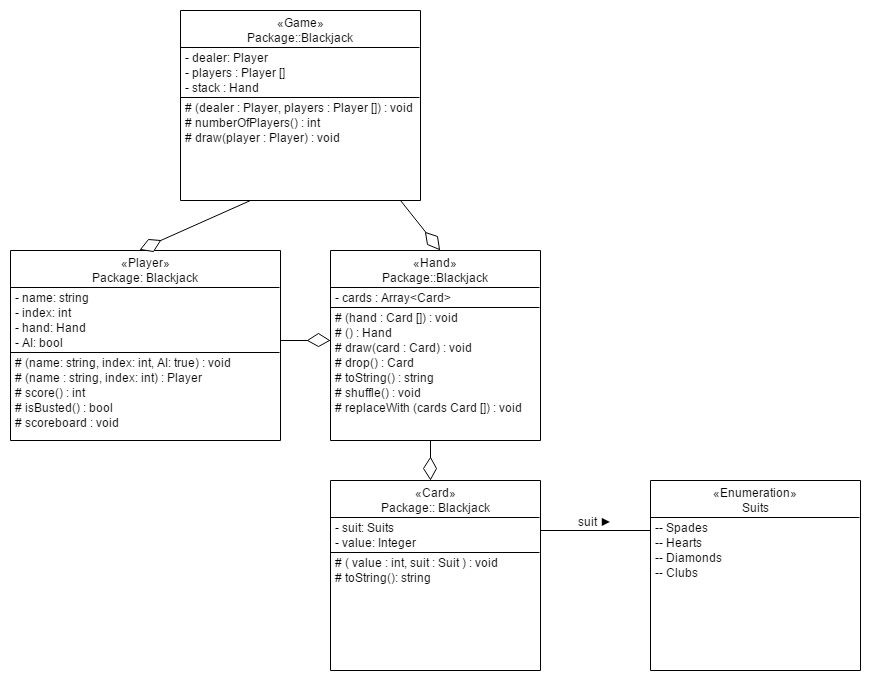
\includegraphics[width=520px]{figures/uml.png}

        \caption{UML diagram over vores klasse implementation}
        \label{fig:umlDiagram}
      \end{figure}

  \section{Programbeskrivelse} \label{sec:programDescription}
    Vores programkode er opdelt i fire filer der kan findes i \path{/src} mappen.
    Filen \path{blackjack.fsx} indeholder spillets hjælpefunktioner, enumerations og klasser,
    der huser de forskellige spilobjekter. Alle disse er beskrevet i Afsnit \ref{sec:design} - \nameref{sec:design}

    Filen \path{game.fsx} indeholder spillets logik, main-loop og det er den files der køres.
    Filen \path{headers.fsx} indeholder headers/"grafik" der printes i konsollen den indeholder følgende headers:
    \begin{enumerate}
      \item menuHeader der vises over hovedmenuen
      \item mainHeader der vises når der skal vælges kommando
      \item header der vises på alle andre tidspunkter
    \end{enumerate}
    Filen \path{tests.fsx} indeholder unit-tests af programmet.

    \subsection{Hjælpefunktioner} \label{ssec:helpers}
      De følgende hjælpefunktioner kan findes i filen \path{/src/blackjack.fsx}, og er relateret til consol-håndtering.
      \begin{description}
      
        \item{\texttt{readln}}~\\
          Alias for \lstinline$System.Console.ReadLine()$
          Der læses en linje fra konsollen og det returneres.

        \item{\texttt{setcursor}}~\\
          Typedefinitionen for funktioen er \lstinline$setcursor(x,y)$.
          Alias for \lstinline$System.Console.SetCursorPosition(x,y)$
          Placere kurseren et bestemt sted i konsollen.

        \item{\texttt{clear}}~\\
          Alias for \lstinline$System.Console.Clear()$.
          Clear tømmer konsollen, så alt indhold fjernes.

        \item{\texttt{write}}~\\
          Typedefinitionen for funktioen er \lstinline$write (str:string)$.
          Alias for \lstinline$System.Console.Write str$
          Der skrives en string ud i konsollen, uden at der tilføjes ekstra nye linjer eller anden formatering.

        \item{\texttt{writeln}}~\\
          Typedefinitionen for funktioen er \lstinline$writeln (str:string)$.
          Alias for \lstinline$System.Console.WriteLine str$.
          Der skrives en linje i konsollen.
      \end{description}~\\
      
      De følgende hjælpefunktioner kan findes i filen \path{/src/game.fsx}, og er relateret til selve game-flowet:
      \begin{description}
        \item{\texttt{validate\_name}}~\\
          Validere om længden af navnet(string) er større end nul,
          og mindre end 25.
      
        \item{\texttt{validate\_yn}}~\\
          Validere om inputtet er i mængden {y, n} af strenge.

        \item{\texttt{printScoreboard}}~\\
          Printer scoreboarded for et spil i konsolen, med den nuværende spiller valgt.
          Hver \texttt{Player} har en scoreboard metode, der printer deres eget scoreboard.
          Denne hjælpefunktion printer derfor først headeren, derefter looper over alle spillerne og printer deres
          og til sidst printes dealerens scoreboard.

        \item{\texttt{selectPlayer}}~\\
          Funktionen tager et \texttt{Player} objekt,
          og så tilføjes der en linje med X'er i konsollen under spillerens scoreboard,
          for at vise at det er den spiller der har tur.

        \item{AI}~\\
          Denne funktion agere AI logik for de spillere der er flagged det.
          Systemet er delt op i nogle forskellige trin.

          \begin{enumerate}
            \item Først beregnes værdien af den spiller der har højest værdi under 22
            \item Så venter systemet 500ms for at simulere lidt menneskelig tænketid
            \item Så beregnes differencen mellem 21 og AI'ens score (den kalder vi diff)
            \item Derefter tælles antal S'er der ikke er i brug
            \item Dernæst tælles antal kort, ikke i brug, $value \leq diff$
          \end{enumerate}

          Når ovenstående trin er gjort, kommer selve stadiet hvor der skal tages et valg.
          For at AI'en vælger at tage et kort til, skal en af følgende være opfyldt.

          \begin{itemize}
            \item Der er 31 eller flere kort $value \leq diff$
            \item Hvis AI har min et es og der er 21 eller flere kort <= diff
            \item Hvis AI ligger under 4 point under den bedste spiller og der er 26 eller flere kort hvor $value \leq diff$,
            dette er for at simulere Human Stupidity eller Daredevils.
          \end{itemize}

          Til sidst printes scoreboardet for spillet og spilleren markeres som stadigvæk at have tur.
      \end{description}
      
    \subsection{Klasser} \label{ssec:classes}
      \begin{description}
        \item{\texttt{\texttt{Card}}}~\\
          Som beskrevet i \namedref{sec:design}, repræsenterer \texttt{Card} et kort ved at indeholde en kulør og en værdi.
          
        \item{\texttt{\texttt{Hand}}}~\\
        \item{\texttt{\texttt{Player}}}~\\
        \item{\texttt{Game}}~\\
      \end{description}
    
    \subsection{Loops} \label{ssec:loops}
    \begin{description}
      \item{\texttt{menu}}~\\
      Menufunktionen holder styr på hovedmenuen, den er vist i \lstinline$menuHeader$.
      Når menuen vises, fjernes alt det der tidligere har været i konsollen.
      Denne menu giver spilleren to muligheder:
      \begin{itemize}
        \item 1 - New game, setup() og menu() kaldes
        \item 2 - Exit game
      \end{itemize}
      De kan vælges ved at bruge taster "1" eller "2".
      
      \item{\texttt{setup}}~\\
      Setup funktionen håndtere start af et nyt spil.
      
      \item{\texttt{main}}~\\
    \end{description}
      
      
  \section{Afprøvning} \label{sec:unitTest}
    Til at sørge for at vores funktioner virker korrekt har vi
    anvendt unit-testing på klasserne Card, Player og Hand.
    Disse tests findes i filen \path{src/tests.fsx}, som skal
    compiles med symbolet TEST, hvilket kan gøres med
    kommandolinjeflaget -d:TEST og derefter kan køres i en
    terminal, hvor der angives true eller false for hver test
    der udføres, hvor true angiver at testen har givet det
    forventede resultat og false angiver en fejl i koden.

	\section{Diskussion og konlusion} \label{sec:conclusion}
    Dette afsnit vil opsummere resultaterne for vores projekt og proceessen vi har været igennem.

    I dette projekt har vi arbejdet ud fra nogle stillede hårde krav (Se \namedref{ssec:demands}),
    og pga det kan resultatet af dette projekt måles direkte - ved at kigge på dem.

    Klassestrukturen er designet ved hjælp af et UML-diagram, vist i \namedref{sec:design},
    og designet følger de fysiske elementer.

    Vores egen problemformulering, som vi har formuleret og nu vil konkludere kan ses i \namedref{sec:problem}.
    Vi har i dette projekt udviklet et spil der følger reglerne for SimpleJack i F\# (Se \namedref{sec:programDescription} og \namedref{sec:unitTest}).
    Spillet kan spilles af 1-5 spillere, eksklusiv dealeren, og det er muligt at have AI spillere.
    Spillet kan også spilles af spillere gennem kommandopromten, som ønsket.

    Programmet er unittestet(Se \namedref{sec:unitTest}), dokumenteret efter XML-standarden og kan kompileres med fsharpc og køres med mono.
  \newpage
  
  \section{Bilag}
      Dette afsnit indeholder en brugervejledning for brug og spil af SimpleJack og spillets programkode.

      \subsection{Brugervejledning} \label{ssec:manual}
        Dette afsnit vil være en step-by-step guide til brug af det udviklede program,
        det skal ikke ses som en vejledning til at spille SimpleJack. Her findes altså ikke nogle regler
        i dette afsnit, men de kan ses i Afsnit \namedref{ssec:demands}.

        Spillet startes ved at køre filen \path{src/game.exe}. \\
        
        Det første det vises vil være spillets hovedmenu, der kan ses i \namedref{fig:mainMenu}.
        I hovedmenuen er der følgende to muligheder:
        \begin{itemize}
          \item 1 - Start nyt spil
          \item 2 - Afslut programmet
        \end{itemize}
        De kan vælges ved at skrive numrene i kommandopromten.

        Hvis mulighed nummer et vælges, begyndes et nyt spil og antal spillere skal vælges (Se \namedref{fig:selectPlayers}).
        Dette tal inkludere AI spillere, men er eksklusivt dealeren.

        Når antal spillere er valgt, vil der for hver spiller være krævet to inputs,
        først "navn" og derefter om spilleren er AI.
        Disse to skræme kan ses i \namedref{fig:selectPlayerName} og \namedref{fig:selectPlayerIsHuman}.

        Nu er spillet klar til at gå i gang, og den første spiller starter.
        Alle spillere starter med 2 kort.
        Den nuværende spiller er markeret med en række af X'er. (Se \namedref{fig:scoreboardDealed}).

        Den nuværende spiller kan nu vælge mellem to kommandoer:
        - Hvis summen af en spillers kort er 21 eller større, gives turen videre.
        \begin{enumerate}
          \item \"hit\" - Trækker et nyt kort
          \item \"stand\" - Giver turen videre (Se \namedref{fig:player3Turn})
        \end{enumerate}

        AI spillere har et delay mellem hver af deres kommandoer, så det føles virkeligt.

        Når alle spillerene har haft tur, er det dealerens tur og efter et lille delay kan spillet afgøres.
        Herefter annonceres vinder(ne)(Se \namedref{fig:winnerIsFound}).

      \subsection{Kildekode} \label{ssec:sourceCode}
        Dette afsnit indeholder alt den kode der er blevet udviklet til projektet,
        både klasser, spillogik og tests.

        \lstinputlisting[caption={Spilklasser},label={lst:blackjack}]{code/blackjack.fsx}
        \lstinputlisting[caption={Spillogikken},label={lst:game}]{code/game.fsx}
        \lstinputlisting[caption={Tests},label={lst:tests}]{../src/tests.fsx}

      \subsection{Billeder}
        Dette afsnit indeholder billeder brugt i de forskellige afsnit,
        der enten er for store til afsnittet eller skal bruges flere steder.

        \begin{figure}[H]
          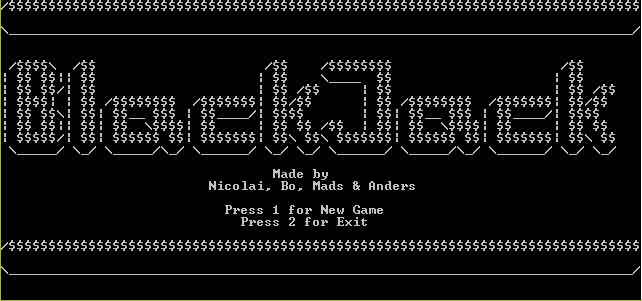
\includegraphics{figures/MainMenu.PNG}

          \caption{Spillets hovedmenu}
          \label{fig:mainMenu}
        \end{figure}

        \begin{figure}[H]
          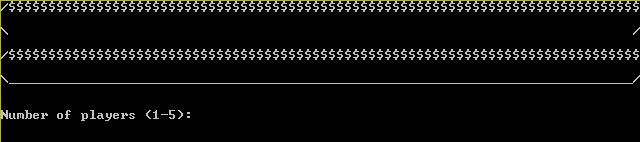
\includegraphics{figures/SelectPlayers.PNG}

          \caption{Vælg antal spillere}
          \label{fig:selectPlayers}
        \end{figure}

        \begin{figure}[H]
          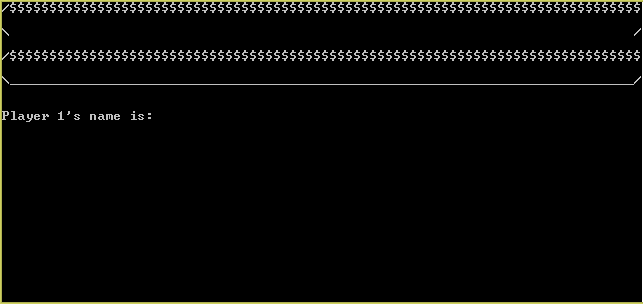
\includegraphics{figures/PlayerName.PNG}

          \caption{Vælg spillers navn}
          \label{fig:selectPlayerName}
        \end{figure}

        \begin{figure}[H]
          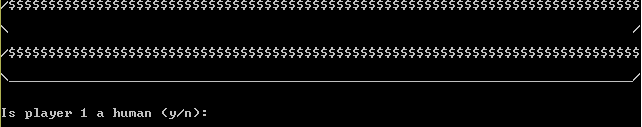
\includegraphics{figures/PlayerIsHuman.PNG}

          \caption{Vælg om spiller er AI eller menneske}
          \label{fig:selectPlayerIsHuman}
        \end{figure}

        \begin{figure}[H]
          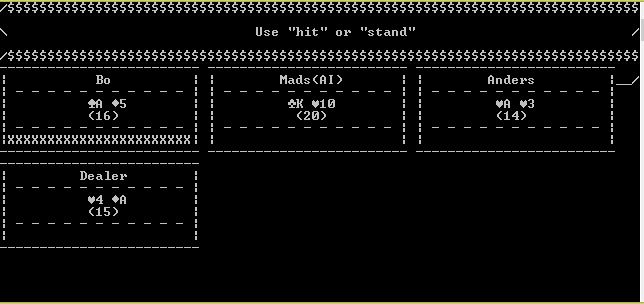
\includegraphics{figures/ScoreBoardDealed.PNG}

          \caption{Spillet starter}
          \label{fig:scoreboardDealed}
        \end{figure}

        \begin{figure}[H]
          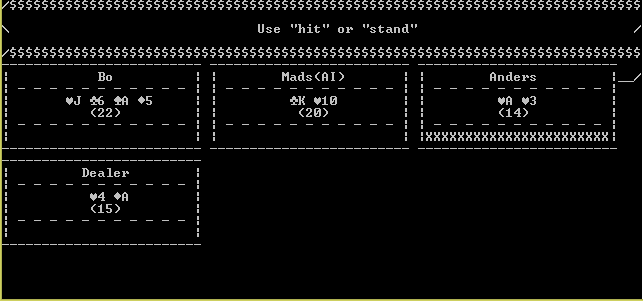
\includegraphics{figures/Player3Playing.PNG}

          \caption{Spiller 3's tur}
          \label{fig:player3Turn}
        \end{figure}

        \begin{figure}[H]
          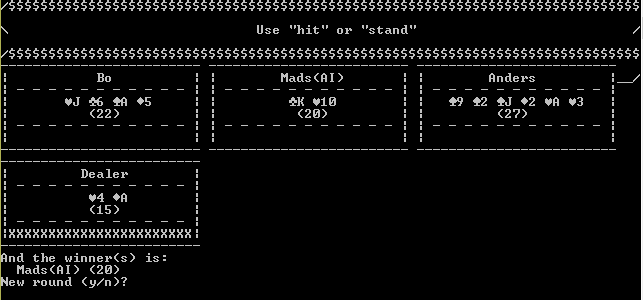
\includegraphics{figures/WinnerIs.PNG}

          \caption{Vinderen er fundet}
          \label{fig:winnerIsFound}
        \end{figure}
\end{document}